\chapter{Quantum Electrodynamics}

The Lagrangian for quantum electrodynamics is
\begin{equation}
\begin{aligned}
	\mathcal{L}_{\mathrm{QED}}
	&= \bar\psi \left(i\gamma^\mu \partial_\mu - m\right)\psi - \frac{1}{4}F_{\mu\nu}F^{\mu\nu} -eA_\mu \bar\psi\gamma^\mu  \psi \\
	&= \mathcal{L}_{\mathrm{Dirac}}+\mathcal{L}_{\mathrm{Maxwell}}+\mathcal{L}_{\mathrm{int}},
\end{aligned}
\end{equation}
where
\begin{equation}
	F_{\mu\nu} = \partial_\mu A_\nu - \partial_\nu A_\nu = (dA)_{\mu\nu}.
\end{equation}
The Lagrangian is invariant under the gauge transformation:
\begin{equation}
\begin{aligned}
	\psi(x) &\rightarrow e^{-ie\alpha(x)}\psi(x), \\
	A^\mu(x) &\rightarrow A^\mu(x) + \partial^\mu \alpha(x).
\end{aligned}
\end{equation}
It is convenient to rewrite Lagrangian as
\begin{equation}
	\mathcal{L}_{\mathrm{QED}}
	= \bar\psi \left(i\cancel{D} - m\right)\psi - \frac{1}{4}F_{\mu\nu}F^{\mu\nu},
\end{equation}
where we have define the covariant derivative as:
\begin{equation}
	\cancel{D} = \gamma^\mu D_\mu 
	= \gamma^\mu [\partial_\mu + i e A_\mu(x)]
	= \cancel{\partial} + ie \cancel{A}.
\end{equation}
As with the scalar field, the partition function with source is defined as
\begin{equation}
	Z[\bar\eta,\eta,J] = \exp\left\{i\int d^dx \mathcal{L}_{\mathrm{int}}\left[\frac{\delta}{i\delta J},\frac{\delta}{i\delta \eta},\frac{i\delta}{\delta \bar\eta}\right]\right\} Z_0[\bar\eta,\eta,J].
\end{equation}
In the following, we will use the dimensional regularization by default. 
Note that the mass dimensionality for the fermion and gauge field is
\begin{equation*}
	[\psi] = \left[\frac{d-1}{2}\right],\quad
	[A] = \left[\frac{d}{2}-1\right],
\end{equation*}
which lead to the coupling constant $e$ to have the dimension
\begin{equation*}
	[e] = \left[2-\frac{d}{2} \right].
\end{equation*}
When $d=4-\epsilon$, we make the replacement
\begin{equation*}
	e \rightarrow e \tilde{\mu}^{\epsilon/2},
\end{equation*}
so that to make the coupling constant $e$ dimensionless.



\section{Perturbative Renormalization}

The interaction will renormalize the field and coefficients to
\begin{equation}
\begin{aligned}
	\psi &= \sqrt{Z_\psi} \psi_R, & m &= Z_m m_R, \\
	A &= \sqrt{Z_A} A_R, & e &= Z_e e_R.
\end{aligned}
\end{equation}
The renormalized Lagrangian is
\begin{equation}
\begin{aligned}
	\mathcal L 
		&= Z_{\psi} \bar\psi_R(i\gamma^\mu \partial_\mu)\psi_R 
		-Z_m Z_\psi m_R \bar\psi_R\psi_R 
		+ Z_{A} \frac{1}{4} F_{R,\mu\nu}F_R^{\mu\nu} - Z_e Z_\psi \sqrt{Z_A} e_R A_R^\mu \bar\psi_R\gamma^\mu \psi_R \\
		&= \mathcal{L}_0 + \mathcal{L}_{\mathrm{int}} + \mathcal{L}_{\mathrm{ct}}.
\end{aligned}
\end{equation}
The we define the coefficients
\begin{equation}
	\delta_{\psi} = Z_\phi - 1,\quad 
	\delta_{m} = Z_m - 1,\quad 
	\delta_A = Z_A - 1, \quad 
	\delta_1 = Z_e Z_\psi \sqrt{Z_A} - 1.
\end{equation}
The counter term also contribute to the perturbative expansion like the interactions.
The counter terms for the fermion propagator come from the diagram expression:
\begin{equation}
\begin{aligned}
	iG_F^{\mathrm{(ct)}}(p)
	&= 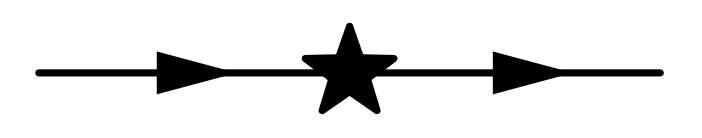
\includegraphics[align=c, width=0.25\linewidth]{pics/QED-ct-1.png} \\
	&= G_F^{(0)}(p) \left[ \delta_{\psi}\cancel{p}-(\delta_m + \delta_\psi) m_R\right] G^{(0)}_F(p) .
\end{aligned}
\end{equation}
The contribution to the electron self energy is
\begin{equation}
	i\Sigma^{(\mathrm{ct})}(p) \equiv \delta_{\psi}\cancel{p}-(\delta_m + \delta_\psi) m_R.
\end{equation}

Similarly, the counter term contribution to the photon self energy is
\begin{equation}
\begin{aligned}
	i \Pi^{(
	\mathrm{ct})}_{\mu\nu}(k) 
	&= 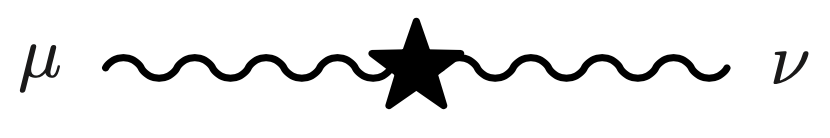
\includegraphics[align=c,width=0.25\linewidth]{pics/QED-ct-2.png} \\
	&= \delta_A [-p^2 g_{\mu\nu} + (1-\xi)p_\mu p_\nu].
\end{aligned}
\end{equation}
In Landau gauge, $\xi=1$ and we can ignore the $p_\mu p_\nu$ terms, and the photon self-energy is always proportional to $g_{\mu\nu}$.
Whenever other gauge choices are concerned, we can simply replace $g_{\mu\nu}$ with
$g_{\mu\nu} - (1-\xi)\frac{p_\mu p_\nu}{p^2}$.

The counter term contribution to the QED vertex is
\begin{equation}
	\Gamma^{\mathrm{(ct)}\mu}_{\alpha\beta} 
	= 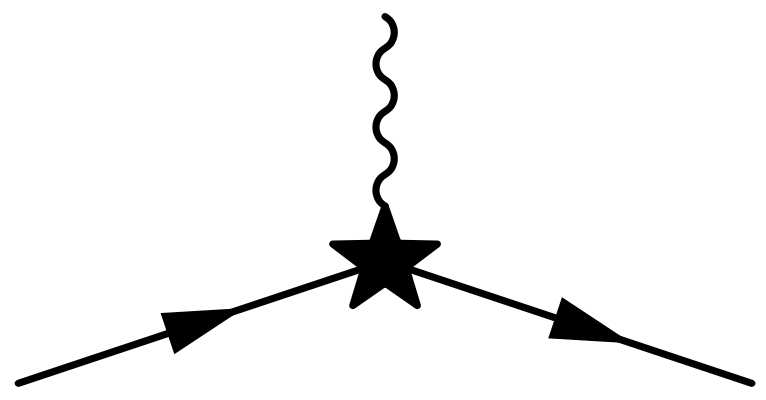
\includegraphics[align=c, width=0.2\linewidth]{pics/QED-ct-3.png} 
	= -\delta_1 \gamma^{\mu}_{\alpha\beta}.
\end{equation}



\subsection{Vacuum Polarization}

Consider the one-loop correction to the photon propagator:
\begin{equation}
\begin{aligned}
	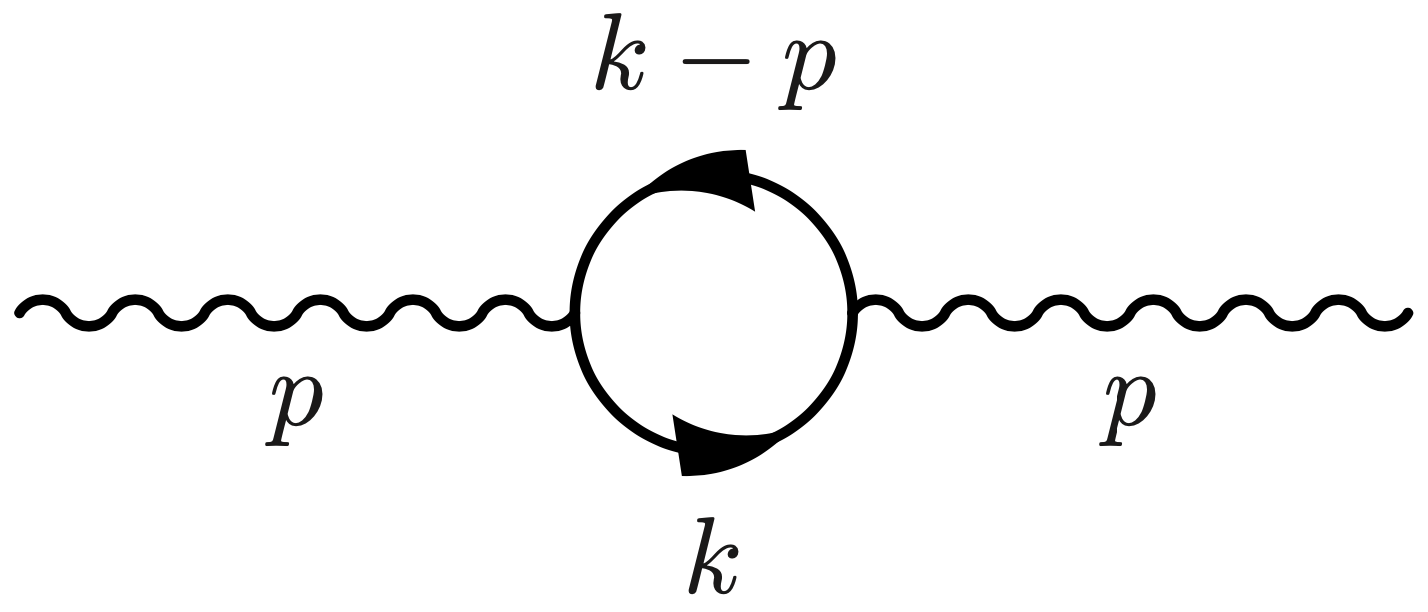
\includegraphics[align=c,width=0.15\linewidth]{pics/QED-2.png} 
	&\simeq (-ie_R)^2\wick{
		A_\mu \c2{\bar\psi}_\alpha \gamma^\mu_{\alpha\beta} \c1{\psi}_\beta 
		A_\nu \c1{\bar\psi}_\gamma \gamma^\nu_{\gamma\tau} \c2{\psi}_\tau
	} \\
	&\equiv iA_\mu \Pi^{\mu\nu}(p) A_\nu.
\end{aligned}
\end{equation}
The self energy is:
\begin{equation}
\begin{aligned}
	i\Pi^{\mu\nu}(p) 
	&= -e_R^2 \int\frac{d^4 k}{(2\pi)^4} \mathrm{Tr}\left[\gamma^\mu G^{(0)}_F(k-p) \gamma^\nu G^{(0)}_F(k) \right] \\
	&= -e_R^2 \int\frac{d^4 k}{(2\pi)^4} 
	\frac{\mathrm{Tr}\left[\gamma^\mu (\cancel k- \cancel p +m_R) \gamma^\nu (\cancel k +m) \right]}{(k^2-m_R^2)[(p-k)^2-m_R^2]}.
\end{aligned}
\end{equation}

The trace of the Dirac matrices can be evaluated in \texttt{Mathematic} using the \texttt{FeynCalc} package:

\begin{lstlisting}[style=mathematicaFrameTB]
(*Dirac trace using FeynCalc`*)
res=DiracTrace[GA[\[Mu]].(GS[k-p]+m).GA[\[Nu]].(GS[k]+m)];
DiracSimplify[res]
\end{lstlisting}

The Dirac trace is:
\begin{equation}
\begin{aligned}
	&\ \mathrm{Tr}\left[\gamma^\mu (\cancel k- \cancel p +m_R) \gamma^\nu (\cancel k +m_R) \right] \\
	=&\ 4 \left[g^{\mu\nu} \left(k\cdot p-{k}^2+m_R^2\right)+ 2k^\mu k^\nu - k^\mu p^\nu - p^\mu k^\nu \right].
\end{aligned}
\end{equation}
Using the Feynman parameters, the denominator is:
\begin{equation}
\begin{aligned}
	\frac{1}{(k^2-m_R^2)[(p-k)^2-m_R^2]}
	&= \frac{1}{\left\{[k-p(1-x)]^2-[m_R^2+p^2 x(x-1)]\right\}^2} \\
	&\equiv \frac{1}{\left\{[k-p(1-x)]^2 - D_x \right\}^2}.
\end{aligned}
\end{equation}
Since the Ward identity requires that the $p^\mu$ term in the propagator do not contribute to any scattering process, we then shift $k \rightarrow k + p(1-x)$ and drop all $p^\mu$ linear term. 
The final result is simplified to:
\begin{equation}
\begin{aligned}
	i\Pi^{\mu \nu}(p) 
	&= -4 e_R^{2} \int_0^1 dx
		\int \frac{d^{4} k}{(2 \pi)^{4}}  \frac{2 k^{\mu} k^{\nu}-g^{\mu \nu}\left[k^{2}-x(1-x) p^{2}-m_R^{2}\right]}{\left[k^{2}-D_x \right]^{2}} \\
	&\simeq 4e_R^2 g^{\mu\nu} \int_0^1 dx \int\frac{d^4 k}{(2 \pi)^{4}}  
		\frac{\frac{1}{2}k^{2}-x(1-x) p^{2}-m_R^{2}}{\left[k^{2}-D_x \right]^{2}} \\
	&\simeq -ie_R^2 g^{\mu\nu} \int_0^1 dx\ \frac{\Omega_d \tilde{\mu}^\varepsilon}{(2\pi)^d} \int_0^\infty dk\ k^{d-1} \frac{\left(4-\frac{2}{d} \right) k^{2}+4x(1-x) p^{2}+4m_R^{2}}{\left[k^{2}+D_x\right]^{2}}.
\end{aligned}
\end{equation}
where we have made the Wick rotation, shifted the dimensionality to $(d=4-\varepsilon)$, and made the substitution (since the self-energy $i\Pi^{\mu\nu} \propto g^{\mu\nu}$):
\begin{equation}
	k^\mu k^\nu \rightarrow \frac{1}{d} k^2 g^{\mu\nu}.
\end{equation}

The remaining problem is to regularize and renormalize the divergent integral
\begin{equation}
	I_\varepsilon(x) \equiv \frac{\Omega_{4-\varepsilon} \tilde{\mu}^\varepsilon}{(2\pi)^{4-\varepsilon}} \int_0^\infty dk\ k^{3-\varepsilon} \frac{\left(4-\frac{8}{4-\varepsilon} \right) k^{2}+4x(1-x) p^{2}+4m_R^{2}}{\left[k^{2}+D_x\right]^{2}}.
\end{equation}

\subsubsection{Regularization and Renormalization}
In $(4-\varepsilon)$-dimensional Euclidean space, the integral is convergent.
The $\varepsilon$-expansion is carried out in \texttt{Mathematica} using the following code:

\begin{lstlisting}[style=mathematicaFrameTB]
omg = (2*Pi^(d/2))/(Gamma[d/2]);
cof = \[Mu]^(4-d)*omg/(2*Pi)^d;
nom = k^(d-1)*((4-8/(4-\[Epsilon]))k^2+4x*(1-x)p^2+4m^2);
int = cof*Integrate[nom/(k^2+D)^2,{k,0,Infinity}][[1]];
map = D->m^2-p^2*x*(1-x);
ans = Series[int/.{d->4-\[Epsilon]},{\[Epsilon],0,0}];
ans /. map // Simplify
\end{lstlisting}

The result is
\begin{equation}
	I_\varepsilon(x) = \frac{p^2 x(1-x)}{2\pi^2} \left[\frac{2}{\varepsilon}+\ln\left(\frac{4\pi e^{-\gamma_E} \tilde\mu^2}{m_R^2-p^2 x(1-x)}\right)\right]
\end{equation}
So the photon self-energy is (also denote $\mu^2=4\pi e^{-\gamma_E} \tilde\mu^2$):
\begin{equation}
	\Pi^{\mu\nu}(p) 
	= -\frac{e_R^2 p^2 g^{\mu\nu}}{6\pi^2 \varepsilon} 
	-\frac{e_R^2 p^2 g^{\mu\nu}}{2\pi^2} \int_0^1 dx\ x(1-x)
	\ln\left[\frac{\mu^2}{m_R^2-p^2 x(1-x)}\right]
\end{equation}
The counter term coefficient can be chosen as
\begin{equation}
	\delta_A = -\frac{e_R^2}{6\pi^2 \epsilon}.
\end{equation}
The renormalized photon self-energy is then
\begin{equation}
\begin{aligned}
	\Pi^{\mu\nu}(p) 
	&= -\frac{e_R^2 p^2 g^{\mu\nu}}{2\pi^2} \int_0^1 dx\ x(1-x)
	\ln\left[\frac{\mu^2}{m_R^2-p^2 x(1-x)}\right] \\
	&= \frac{e_R^2 p^2 g^{\mu\nu}}{2\pi^2} \left\{\frac{1}{3}\ln\left(\frac{m_R}{\mu}\right)
	 + \int_0^{1} dx\ x(1-x) \ln\left[1-\frac{p^2 x(1-x)}{m_R^2}\right] \right\}.
\end{aligned}
\end{equation}


\subsubsection{Physical Observable}

The photon self-energy has the form
\begin{equation}
	\Pi^{\mu\nu}(p) = -e_R^2 \left[g^{\mu\nu}-(1-\xi)p^\mu p^\nu\right] g^{\mu\nu} \Pi_2(p),
\end{equation}
where
\begin{equation}
	\Pi_2(p) = \frac{1}{2\pi^2} \int_0^1 dx\ x(1-x)
	\ln\left[\frac{\mu^2}{m_R^2-p^2 x(1-x)}\right]
\end{equation}
The one-loop correction to photon propagator is
\begin{equation}
\begin{aligned}
	iG^{\mu\nu}_\gamma(p) 
	&= -i \frac{g^{\mu\nu}}{p^2} \left(1 + \sum_{n=1}^\infty (-e_R^2)^n \Pi_2^n(p) \right) \\
	&= -i\frac{g^{\mu\nu}}{p^2 \left[1+e_R^2\Pi_2(p) \right]}.
\end{aligned}
\end{equation}

We can choose the on-shell condition that the photon has no rest mass:
\begin{equation}
	\Pi_2(0) = 0 \quad \Longrightarrow \quad
	\mu = m_R.
\end{equation}
Note that the propagator is related to the Coulomb potential.\footnote{The Coulomb potential arises just like we derive the force (\ref{eq:field-to-force}), but the sources have additional charge $e_R$, and the photon is mass less, so $V(p) = \frac{e_R^2}{p^2}$ for free field.
}
To the second order,
\begin{equation}
\begin{aligned}
	V(p) &= e_R^2 \frac{1-e_R^2 \Pi_2(p)}{p^2} + O(e_R^6) \\
	&= \frac{e_R^2}{p^2}\left\{1 + \frac{e_R^2}{2\pi^2}\int_0^1 dx\ x(1-x)\ln\left[1-\frac{p^2 x(1-x)}{m_R^2}\right] + O(e_R^4)\right\}.
\end{aligned}
\end{equation}

Consider the small momentum limit, where the integral in approximated by
\begin{equation}
\begin{aligned}
	\int_0^1 dx\ x(1-x)\ln\left[1-\frac{p^2 x(1-x)}{m_R^2}\right]
	\approx -\frac{p^2}{m_R^2} \int_0^1 dx\ x^2(1-x)^2 = -\frac{p^2}{30 m_R^2}.
\end{aligned}
\end{equation}
This implies
\begin{equation}
	V(p) = \frac{e_R^2}{p^2} - \frac{e_R^4}{60\pi^2 m_R^2}.
\end{equation}
The Fourier transformation gives
\begin{equation}
	V(r) = -\frac{e_R^2}{4\pi r} - \frac{e_R^4}{60\pi^2 m_R^2}\delta^{(3)}(r).
\end{equation}
For atomic orbit, since only the ($L=0$)-orbit have support at $r=0$, this extra potential will shift the spectrum.
This effect is called the \textit{Lamb shift}.

On the other hand, the the large momentum limit,
\begin{equation}
	V(p) \approx \frac{e_R^2}{p^2}\left[ 1 + \frac{e_R^2}{12\pi^2} \ln \frac{-p^2}{m_R^2} \right],
\end{equation}
which predicts a \textit{Landau pole} beyond which perturbation theory breaks down.




\subsection{One-loop Correction to Electron Propagator}

Consider the one-loop correction to the particle propagator:
\begin{equation}
	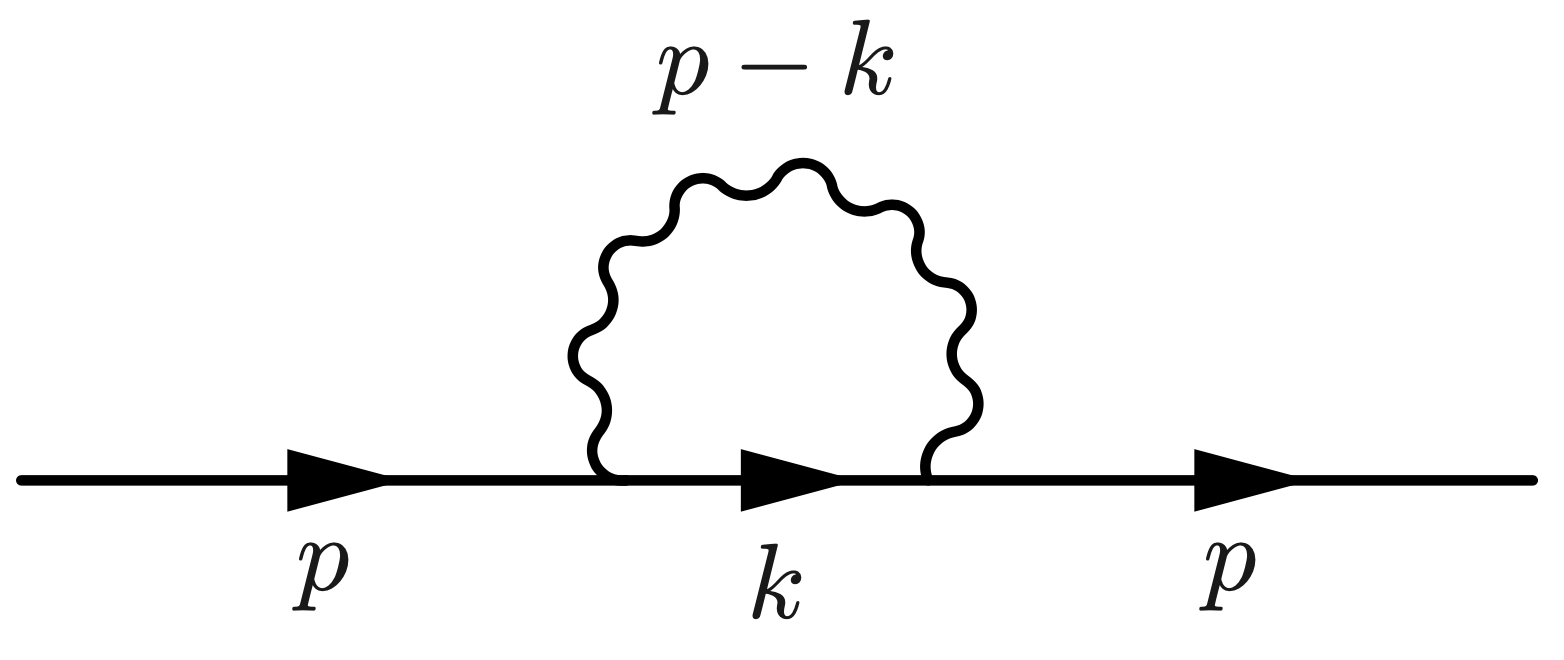
\includegraphics[width=0.2\linewidth,align=c]{pics/QED-1.png} \simeq (-ie_R)^2\wick{
		\c1{A}_\mu \bar\psi_\alpha \gamma^\mu_{\alpha\gamma} \c2{\psi}_\gamma
		\c1{A}_\nu \c2{\bar\psi}_\tau \gamma^\nu_{\tau\beta} \psi_\beta}
	\equiv i\bar\psi_\alpha \Sigma^{\alpha\beta}(p) \psi_\beta.
\end{equation}
The self energy is
\begin{equation}
\begin{aligned}
	i\Sigma_{\alpha\beta}(p)
	&= e_R^2\int\frac{d^4 k}{(2\pi)^4} G^{\mu\nu}_\gamma(p-k) \left[\gamma_\mu G_F(k) \gamma_\nu\right]_{\alpha\beta} \\
	&= -e_R^2\int\frac{d^d k}{(2\pi)^d}\frac{\gamma^\mu(\cancel{k}+m_R)\gamma_\mu}{(p-k)^2(k^2-m_R^2)}.
\end{aligned}
\end{equation}
The seconded equality comes from the contraction:
\begin{equation}
	(-ie)^2\wick{
		\c1{A}_\mu \bar\psi_\alpha \gamma^\mu_{\alpha\gamma} \c2{\psi}_\gamma
		\c1{A}_\nu \c2{\bar\psi}_\tau \gamma^\nu_{\tau\beta} \psi_\beta}
\end{equation}
The nominator can be simplified using the Dirac matrix identities:
\begin{equation}
	\gamma^\mu \gamma_\mu = d, \quad
	\gamma^\mu \gamma^\nu \gamma_\mu = (2-d) \gamma^\nu
	\quad \Longrightarrow \quad
	\gamma^\mu(\cancel{k}+m_R)\gamma_\mu = d m_R+(2-d)\cancel{k}.
\end{equation}
The denominator can be simplify using the Feynman parameter:
\begin{equation}
\begin{aligned}
	\frac{1}{(p-k)^2(k^2-m_R^2)} 
	&= \int_0^1 \frac{dx}{\left[(k-px)^2-(1-x)(m_R^2-p^2 x)\right]^2} \\
	&\rightarrow \int_0^1 \frac{dx}{\left(k^2-D_x\right)^2}
\end{aligned}
\end{equation}
where we have shifted $k \rightarrow k + px$ (note this shift also change the numerator).

The self energy becomes (including a $\tilde \mu$ mass scale):
\begin{equation}
\begin{aligned}
	i\Sigma(p)
	&= e_R^2\tilde{\mu}^{\varepsilon} 
		\int_0^1 [(2-\varepsilon)x\cancel{p}-(4-\varepsilon)m_R] dx 
		\int \frac{d^d k}{(2\pi)^d} 
		\frac{1}{(k^2-D_x)^2} \\
	&= ie_R^2 \int_0^1 dx\ [(2-\varepsilon)x\cancel{p}-(4-\varepsilon)m_R]\ 
		\frac{\tilde{\mu}^{\varepsilon}\Omega_d}{(2\pi)^d} 
		\int \frac{k^{d-1} dk}{(k^2+D_x)^2}.
\end{aligned}
\end{equation}


\subsubsection{Regularization and Renormalization}

The regularization procedure is carried out by the following code:

\begin{lstlisting}[style=mathematicaFrameTB]
omg=(2*Pi^(d/2))/(Gamma[d/2]);
cof=\[Mu]^(4-d)*omg/(2*Pi)^d;
int=cof*Integrate[q^(d-1)/(q^2+D)^2,{q,0,Infinity}][[1]];
map={e->Sqrt[4*Pi*\[Alpha]],EulerGamma->Subscript[\[Gamma],E]};
ans=Series[int/.{d->4-\[Epsilon]},{\[Epsilon],0,0}];
ans/.map//Simplify
\end{lstlisting}

The result is ($\mu^2 = 4\pi e^{-\gamma_E} \tilde\mu^2$)
\begin{equation}
\begin{aligned}
	\Sigma(p) 
	&= \frac{e_R^2}{16\pi^2}\int_0^1 dx \left[(2-\varepsilon)x\cancel{p}-(4-\varepsilon)m_R \right] 
	\left[\frac{2}{\varepsilon}+\ln\frac{\mu^2}{(1-x)(m_R^2-p^2 x)}\right] \\
	&= \frac{e_R^2}{16\pi^2} \left\{ \int_0^1 dx \left[2x\cancel{p}-4m_R \right] 
	\left[\frac{2}{\varepsilon}+\ln\frac{\mu^2}{(1-x)(m_R^2-p^2 x)}\right]-\cancel p + 2m_R\right\}.
\end{aligned}
\end{equation}
The infinity comes from
\begin{equation}
	\frac{e_R^2}{4\pi^2\varepsilon}\int_0^1 dx(x\cancel{p}-2m_R)
	= \frac{e_R^2}{8\pi^2\varepsilon}\cancel{p} - \frac{e_R^2}{2\pi^2\varepsilon}m_R.
\end{equation}
Using the $\overline{\mathrm{MS}}$ subtraction scheme, we choose
\begin{equation}
	\delta_{\psi} = -\frac{e_R^2}{8\pi^2\varepsilon},\quad
	\delta_m = -\frac{3 e_R^2}{8\pi^2\varepsilon},
\end{equation}
and the self energy is
\begin{equation}
	\Sigma(p) 
	= \frac{e_R^2}{16\pi^2} \left\{\int_0^1 dx(2x\cancel{p}-4m_R)\ln\left[\frac{\mu^2}{(1-x)(m_R^2-p^2 x)}\right]-\cancel p + 2m_R \right\}.
\end{equation}


\subsubsection{Physical Observables}

The Dyson series gives:
\begin{equation}
	iG_F(p) = \frac{i}{\cancel p - m_R + \Sigma(p)}
\end{equation}
Experimentally, for a given 
The on-shell subtraction requires that the $m_R$ equals to the physical mass:
\begin{equation}
	\left. \Sigma(\cancel p) \right|_{\cancel p=m_R} = 0, \quad 
	\left. \frac{d}{d \cancel p}\Sigma(\cancel p) \right|_{\cancel p=m_R} = 0.
\end{equation}
To implement the on-shell condition, we have to modify the subtraction scheme to
\begin{equation}
\begin{aligned}
	\delta_{\psi} &= -\frac{e_R^2}{8\pi^2}\left(\frac{1}{\varepsilon}+\ln\frac{\mu}{m_R} +A\right), \\
	\delta_m &= -\frac{e_R^2}{8\pi^2}\left(\frac{3}{\varepsilon} + 3\ln\frac{\mu}{m_R} + B\right),
\end{aligned}
\end{equation}
and the self energy is
\begin{equation}
\begin{aligned}
	\Sigma(\cancel p)
	=&\ -\frac{e_R^2}{8\pi^2} \int_0^1 dx(x\cancel{p}-2m_R)\ln\left[(1-x)\left(1- \frac{p^2}{m_R^2} x \right)\right]\\
	&\  -\frac{e_R^2}{8\pi^2} \left[\left(A+\frac{1}{2}\right)\cancel p - (A+B+1)m_R\right].
\end{aligned}
\end{equation}
The first condition
\begin{equation}
\begin{aligned}
	\left. \Sigma(\cancel p) \right|_{\cancel p=m_R}
	&= -\frac{e_R^2}{8\pi^2} m_R \left[\int_0^1 dx\ (x-2) \ln(1-x)^2 - B-\frac{1}{2}\right] \\
	&= -\frac{e_R^2}{8\pi^2} m_R \left(2 - B\right) = 0
\end{aligned}
\end{equation}
gives the mass renormalization coefficient
\begin{equation}
	\delta_m = -\frac{e_R^2}{8\pi^2}\left(\frac{3}{\varepsilon} + 3\ln\frac{\mu}{m_R} + 2\right).
\end{equation}
While in the derivative of the self-energy:
\begin{equation}
	\frac{d}{d \cancel p}\Sigma(m_R)  
	= -\frac{e_R^2}{8\pi^2} \left\{\int_0^1 dx\ \left[ x\ln(1-x)^2 -\frac{2x(x-2)}{1-x}\ln(1-x)\right] + A + \frac{1}{2}\right\},
\end{equation}
there is a divergent integral:
\begin{equation}
	\int_0^1 dx\ \frac{2x(x-2)}{1-x}\ln(1-x),
\end{equation}
indicating an IR divergence.
We can never the less get rid of it by introducing a small mass $m_\gamma$ for photon (which will be set to zero).
This mass term change the denominator in the loop integral:
\begin{equation}
	\frac{1}{\left[(p-k)^2-m_\gamma^2\right](k^2-m_R^2)} 
	= \int_0^1 \frac{dx}{\left[(k-px)^2-D_x -x m_\gamma^2\right]^2}.
\end{equation}
Most derivation remains the same, we just need to make a substitution in the finial result:
\begin{equation}
	D_x \rightarrow D_x + x m_\gamma^2.
\end{equation}
Especially, the introducing of the photon mass will not change the result of the mass renormalization factor we have computed.

The modified self-energy is then
\begin{equation}
\begin{aligned}
	\Sigma(\cancel p)
	=&\ -\frac{e_R^2}{8\pi^2} \int_0^1 dx(x\cancel{p}-2m_R)\ln\left[(1-x)\left(1- \frac{p^2}{m_R^2} x \right) + x \frac{m_\gamma^2}{m_R^2} \right]\\
	&\  -\frac{e_R^2}{8\pi^2} \left[\left(A+\frac{1}{2}\right)\cancel p - (A+B+1)m_R\right].
\end{aligned}
\end{equation}
The derivative is now
\begin{equation}
	\frac{d}{d \cancel p}\Sigma(m_R)  
	= -\frac{e_R^2}{8\pi^2} \left\{ \int_0^1 dx\ \left[ x\ln(1-x)^2 +\frac{2x(2-x)(1-x)}{(1-x)^2 + x \frac{m_\gamma^2}{m_R^2}} \right] + A + \frac{1}{2}\right\},
\end{equation}
Note that in the ($m_\gamma \rightarrow 0$) limit, the asymptotic behavior of the originally divergent integral is
\begin{equation}
	\lim_{m_\gamma \rightarrow 0} \int_0^1 dx\ \frac{2x(2-x)(1-x)}{(1-x)^2 + x \frac{m_\gamma^2}{m_R^2}}
	= -1 - 2\ln \frac{m_\gamma}{m_R}.
\end{equation}
So the second subtraction condition is:
\begin{equation}
	\frac{d}{d \cancel p}\Sigma(m_R)  
	= -\frac{e_R^2}{8\pi^2} \left(A -2 - 2\frac{m_\gamma}{m_R} \right) = 0.
\end{equation}
The field strength renormalization is
\begin{equation}
	\delta_\psi = -\frac{e_R^2}{8\pi^2}\left(\frac{1}{\varepsilon}+\ln\frac{\mu}{m_R} +2+2\ln\frac{m_\gamma}{m_R}\right).
\end{equation}
The final self energy is (shall take the $m_\gamma \rightarrow 0$ limit):
\begin{equation}
\begin{aligned}
	\Sigma(\cancel p)
	=&\ -\frac{e_R^2}{16\pi^2} \int_0^1 dx(2x\cancel{p}-4m_R)\ln\left[(1-x)\left(1- \frac{p^2}{m_R^2} x \right) + 2x \ln\frac{m_\gamma}{m_R} \right]\\
	&\  -\frac{e_R^2}{16\pi^2} \left[\left(5+4\ln\frac{m_\gamma}{m_R}\right)\cancel p - \left(10 +4\ln\frac{m_\gamma}{m_R}\right)m_R\right].
\end{aligned}
\end{equation}



\subsection{One-loop Correction to Vertex}
Consider the one-loop correction to interaction:
\begin{equation}
\begin{aligned}
	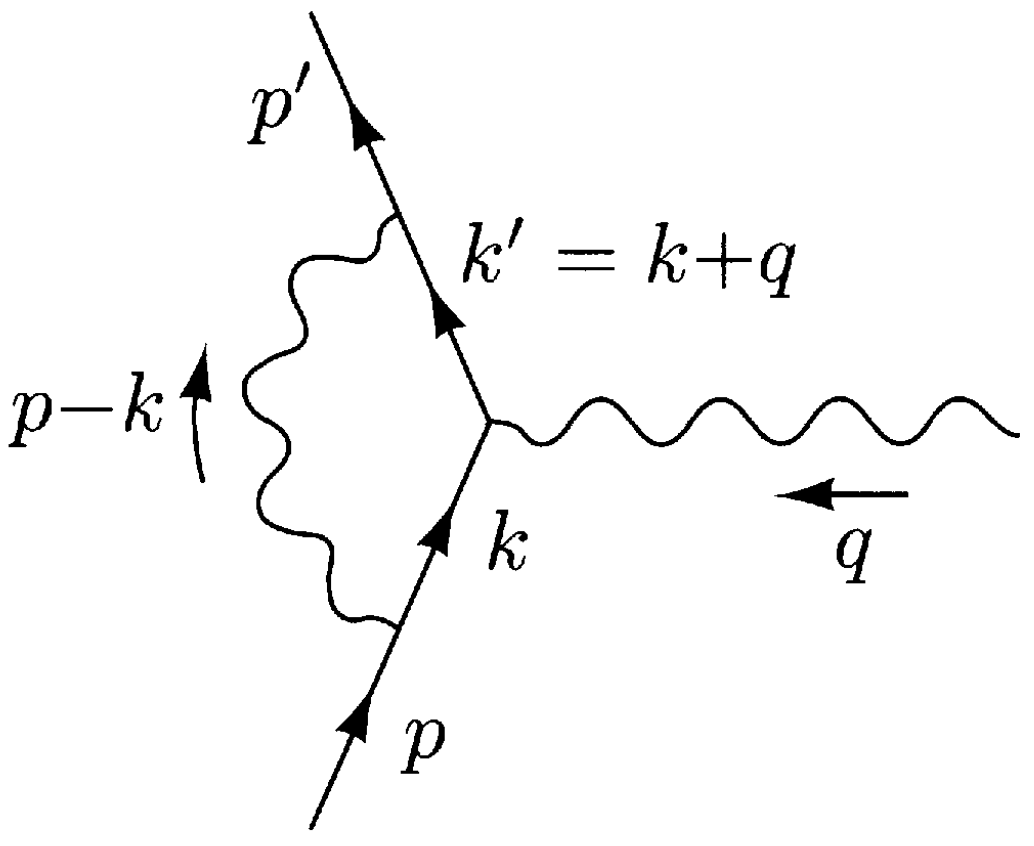
\includegraphics[align=c,width=0.23\linewidth]{pics/QED-3.png}
	& \simeq (-ie_R)^3\wick{
		\c1{A}_\nu \bar\psi_\alpha \gamma^\nu_{\alpha\beta} \c2{\psi}_\beta 
		A_\mu \c2{\bar\psi}_\lambda \gamma^\mu_{\lambda\tau} \c3{\psi}_\tau
		\c1{A}_\xi \c3{\bar\psi}_\rho \gamma^\nu_{\rho\sigma} \psi_\sigma
	} \\ &\equiv -ie A_\mu \Gamma^\mu_{\alpha\beta}(q,p,p') \bar\psi_\alpha \psi_\beta.
\end{aligned}
\end{equation}
The vertex function is:
\begin{equation}
\begin{aligned}
	i\Gamma^\mu_{\alpha\beta}(q,p,p')
	&= -e_R^2 \int\frac{d^4 k}{(2\pi)^4} 
	G_\gamma^{\nu\lambda}(p-k) 
	[\gamma_\nu G_F(k') \gamma^\mu G_F(k) \gamma_\lambda]_{\alpha\beta} \\
	&= e_R^2 \int\frac{d^4 k}{(2\pi)^4} 
	\frac{[\gamma^\nu(\cancel{k}'+m_R)\gamma^\mu (\cancel{k}+m_R)\gamma_\nu]_{\alpha\beta}}{(k^2-m_R^2)(k'^2-m_R^2)(p-k)^2}
\end{aligned}
	\label{eq:QED-loop-vertex}
\end{equation}
Using the following code
\begin{lstlisting}[style=mathematicaFrameTB]
(*numerator*)
den=Contract[GA[\[Nu]].(GS[kp]+m).GA[\[Mu]].(GS[k]+m).GA[\[Nu]]];
DiracSimplify[den]

(*Feynman parameter*)
A1=k^2-m^2;
A2=(k+q)^2-m^2;
A3=(p-k)^2;
{c,b,a}=CoefficientList[x*A1+y*A2+z*A3,{k}];
-b/2//Simplify
-c+b^2/4//Simplify
\end{lstlisting}
The numerator is
\begin{equation}
	-2\cancel{k}\gamma^\mu\cancel{k}'-2m_R^2\gamma^\mu + 4m_R(k + k')^\mu.
\end{equation}
The denominator is
\begin{equation}
	\int \frac{dF_3}{[(k+yq-zp)^2-D_{xyz}]^3},
\end{equation}
where 
\begin{equation*}
\begin{aligned}
	D_{xyz} &= (x+y)m^2 - z(1-z)p^2- y(1-y)q^2-2yzpq \\
	&=(x+y)m_R^2 - xy q^2- yz p'^2 - xz p^2.
\end{aligned}
\end{equation*}
Shift $k^\mu \rightarrow k^\mu + z q_1^\mu - y p^\mu$, throw away all terms with linear $k^\mu$, and replace $k^\mu k^\nu$ with $\frac{1}{d}k^2 g^{\mu\nu}$, the result is
\begin{equation*}
	\frac{4}{d}k^2\gamma^\mu  -2(-y \cancel{q}+z \cancel{p}) \gamma^{\mu}[(1-y) \cancel q+z \cancel p] +4 m_R^{2} \gamma^{\mu}-2 m_R\left[(1-2 y) q^{\mu}+2 z p^{\mu}\right].
\end{equation*}
Note that only the quadratic term is divergent. 
\begin{equation*}
	\Gamma^\mu(p,q_1,q_2) = -i\frac{4e^2\tilde{\mu}^{\epsilon} \gamma^\mu}{d}  \int dF_3 \int \frac{d^dk}{(2\pi)^d} \frac{k^2}{(k^2-D)^3} + \delta\Gamma^\mu(p,q_1,q_2).
\end{equation*}
where $\delta \Gamma^\mu$ stores all the finite part
\begin{equation*}
\begin{aligned}
	& \delta\Gamma^\mu(p,q_1,q_2) \\
	=& \int \frac{e^2 k^3 dk dF_3}{(2\pi)^2(k^2+D)^3} \left\{(-y \cancel{q}+z \cancel{p}) \gamma^{\mu}[(1-y) \cancel q+z \cancel p] -2 m_R^{2} \gamma^{\mu}+ m_R\left[(1-2 y) q^{\mu}+2 z p^{\mu}\right]\right\}.
\end{aligned}
\end{equation*}
The divergent part is
\begin{equation}
	\frac{4 e^2\tilde{\mu}^{\epsilon} \Omega_d \gamma^\mu}{d(2\pi)^d}\int dF_3 \int \frac{k^{d+1}dk}{(k^2+D)^3}
	= \frac{e_R^2}{16\pi^2} \gamma^\mu \int dF_3 \left(\frac{2}{\epsilon}+\ln\frac{\mu^2}{D_{xyz}}\right).
\end{equation}
Using the $\overline{\mathrm{MS}}$ scheme, the coefficient of the counter term is
\begin{equation}
	\delta_e = -\frac{e_R^2}{8\pi^2\varepsilon}.
\end{equation}



\section{Systematic Renormalization}



\subsection{Renormalization Group}
In summery, the renormalization factors are
\begin{equation}
\begin{aligned}
	Z_\psi &= 1 -\frac{e_R^2}{8\pi^2\epsilon} + O(e_R^3), \\
	Z_A &= 1 - \frac{e_R^2}{6\pi^2 \epsilon} + O(e_R^3), \\
	Z_m &= 1 - \frac{e_R^2}{2\pi^2\epsilon} + O(e_R^3), \\
	Z_e &= 1 - \frac{e_R^2}{8\pi^2\epsilon} + O(e_R^3),
\end{aligned}
\end{equation}
which means
\begin{equation}
\begin{aligned}
	\frac{d\ln Z_\phi}{d e_R} &= -\frac{e_R}{4\pi^2 \epsilon} + O(e_R^2), \\
	\frac{d\ln Z_A}{d e_R} &= -\frac{e_R}{3\pi^2 \epsilon} + O(e_R^2), \\
	\frac{d\ln Z_m}{d e_R} &= -\frac{e_R}{\pi^2 \epsilon} + O(e_R^2), \\
	\frac{d\ln Z_e}{d e_R} &= -\frac{e_R}{4\pi^2 \epsilon} + O(e_R^2).
\end{aligned}
\end{equation}
The bare parameters are
\begin{equation}
\begin{aligned}
	\psi_0 &= Z_\psi^{1/2}\psi_R, \\
	A_0 &= Z_A^{1/2} A_R, \\
	m_0 &= Z_m Z_\psi^{-1} m_R, \\
	e_0 &= Z_e Z_\psi^{-1} Z_A^{-1/2} e_R \tilde{\mu}^{\epsilon/2}. 
\end{aligned}
\end{equation}
The RG equation for $e_0$ is
\begin{equation}
	\frac{d\ln e_0}{d\ln \mu}
	= \left(\frac{\ln Z_e}{d e_R} - \frac{\ln Z_\psi}{d e_R} - \frac{1}{2} \frac{\ln Z_A}{d e_R} + \frac{1}{e_R} \right)\frac{de_R}{d\ln \mu} + \frac{\epsilon}{2} = 0.
\end{equation}
The beta function is
\begin{equation}
	\beta(e_R) = \frac{de_R}{d\ln \mu} = -\frac{\epsilon}{2}e_R + \frac{e_R^3}{12\pi^2} + O(e_R^4).
\end{equation}
The RG equation for $m_0$ is
\begin{equation}
	\frac{d\ln m_0}{d\ln \mu}
	= \left(\frac{\ln Z_m}{d e_R} - \frac{\ln Z_\psi}{d e_R}\right)\frac{de_R}{d\ln \mu} + + \frac{1}{m_R}\frac{d m_R}{d\ln\mu} = 0.
\end{equation}
The anomalous dimension of mass is
\begin{equation}
	\gamma_m = \frac{d \ln m_R}{d\ln\mu} = -\frac{3e_R^2}{8\pi^2} + O(e_R^3).
\end{equation}



